  On remarque que sur les courbes des projections de l'image en X et en Y, la courbe marque des paliers au 
niveau des carrés du \rubic{}. 

  Étant donné que la couleur est fortement corrélée sur ces paliers, nous avons décidé d'étudier la variance sur 
un nombre défini de points successifs de ces courbes et d'en extraire des plats caractéristiques de ces paliers. 

\subsubsection*{Principe de la méthode} 

  Cette méthode étudie la variance des vecteurs de projection en X et Y de l'image. 

Afin de la mettre en place, nous avons créé une méthode intermédiaire qui permet de calculer un vecteur contenant les valeurs de la variance 
du vecteur en entrée sur un nombre de points successifs défini. 

La méthode générale suit les étapes suivantes : 
\begin{enumerate}
  \item Calcule de la variance du vecteur de projection en entrée grâce à la fonction décrite précédement. 
  \item Recherche du seuil tel que l'on ait un nombre de plat calculé inférieur ou égal à un nombre voulu. 

Nous faisons le choix d'initialiser un seuil à $\frac{1}{4}$ de la valeur maximale du vecteur en entrée 
et de fixer le pas de modification de ce seuil à $-\frac{1}{10}$ de cette valeur. 
%On initialise la valeur de retour de façon a ce qu'elle vérifie la condition d'entrée dans l'itération suivante : 
\begin{itemize}
  \item On note X la largeur maximale d'un plat. 
Afin d'optimiser l'algorithme et pour garantir une distance minimum entre les plats recherchés, nous avons 
établi que l'indice de parcours de la variance étudiée commence à X et avance par pas de $\frac{X}{2}$ jusqu'à la fin du vecteur 
variance moins la valeur $\frac{X}{2}$. 
  \item On considère qu'un plat existe quand la moyenne de X valeurs successives du vecteur de variance est inférieure au seuil. 
Nous concervons dans un vecteur les indices vérifiant cette condition.
La taille de ce vecteur est la condition de sortie de l'itération.  
  \item Le seuil est diminué de la valeur d'un pas de seuil à chaque itération. 
\end{itemize}

  \item Si le nombre de plat contenus dans le vecteur est égal au nombre voulu, on a le résultat ; 
Sinon, nous récupérons la valeur du vecteur contenant les indices des plats à l'itération précédente et 
nous y supprimons successivement les valeurs les plus semblables aux autres afin d'avoir le nombre de plats souhaité. 

  La distance que nous avons choisi pour calculer la matrice de distance entre ces valeurs et déterminer leur pertinence,
est la distance euclidienne. 
\end{enumerate}

  Les signatures des fonctions créées sont les suivantes : 
\begin{itemize}
  \item \textit{function [variancefinale] = varianceCoordonnee(vecteur, longueurVariance)}
  \item \textit{function [plat] = detectionPlatVariance1D(vecteur, longueurVariance, nombreDePlat, largeurPlat)}
\end{itemize}

\subsubsection*{Résultats obtenus par cette méthode}

     La figure~\ref{variance_resultat_1} présente le résultat obtenu sur une image orientée et ayant subit un filtrage avec la méthode de la variance 1D : 
 
 \begin{figure}[!h]
 \centering
 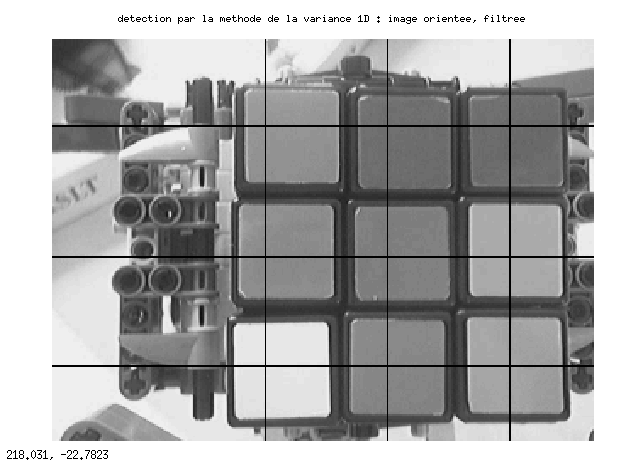
\includegraphics[width=0.9\linewidth]{Images/Variance1D_img_traitement.png} 
 \caption{Résultat de la méthode variance 1D} 
 \label{variance_resultat_1}
 \end{figure}
